\documentclass{article}
\title{CS 205 Homework 5}
\author{Keith Lehman, kpl56@scarletmail.rutgers.edu}

\usepackage[margin=0.5in]{geometry}
\usepackage{graphicx}
\usepackage{amssymb}

\begin{document}
\maketitle

\begin{enumerate}

\item Given an arbitrary relation $R$, suppose we compute two new relations. Prove $R_{1} = R_{2}$ for all $R$. \\
For $R_{1}$ to be the reflixive closure of the transitive closure of $R$, it first must have every element map to the next element and every succeeding element. For it to be reflexive, each element mentioned must also be related to itself. For $R_{2}$ to be the transitive closure of the reflexive closure of $R$, it first must have every element related to itself, then, for each element, it must relate to the following element, as well as every other following element. Under these conditions, both $R_{1}$ and $R_{2}$ will continue the exact same elements. 

\item Let $ A = $ \{cat, dog, bird, rat\} and $R$ be a relation on $A$ defined by \{$(x,y): x$ and $y$ have at least one letter in common\}. \\
\begin{enumerate}
\item  Draw $R$ as a directed graph. \\
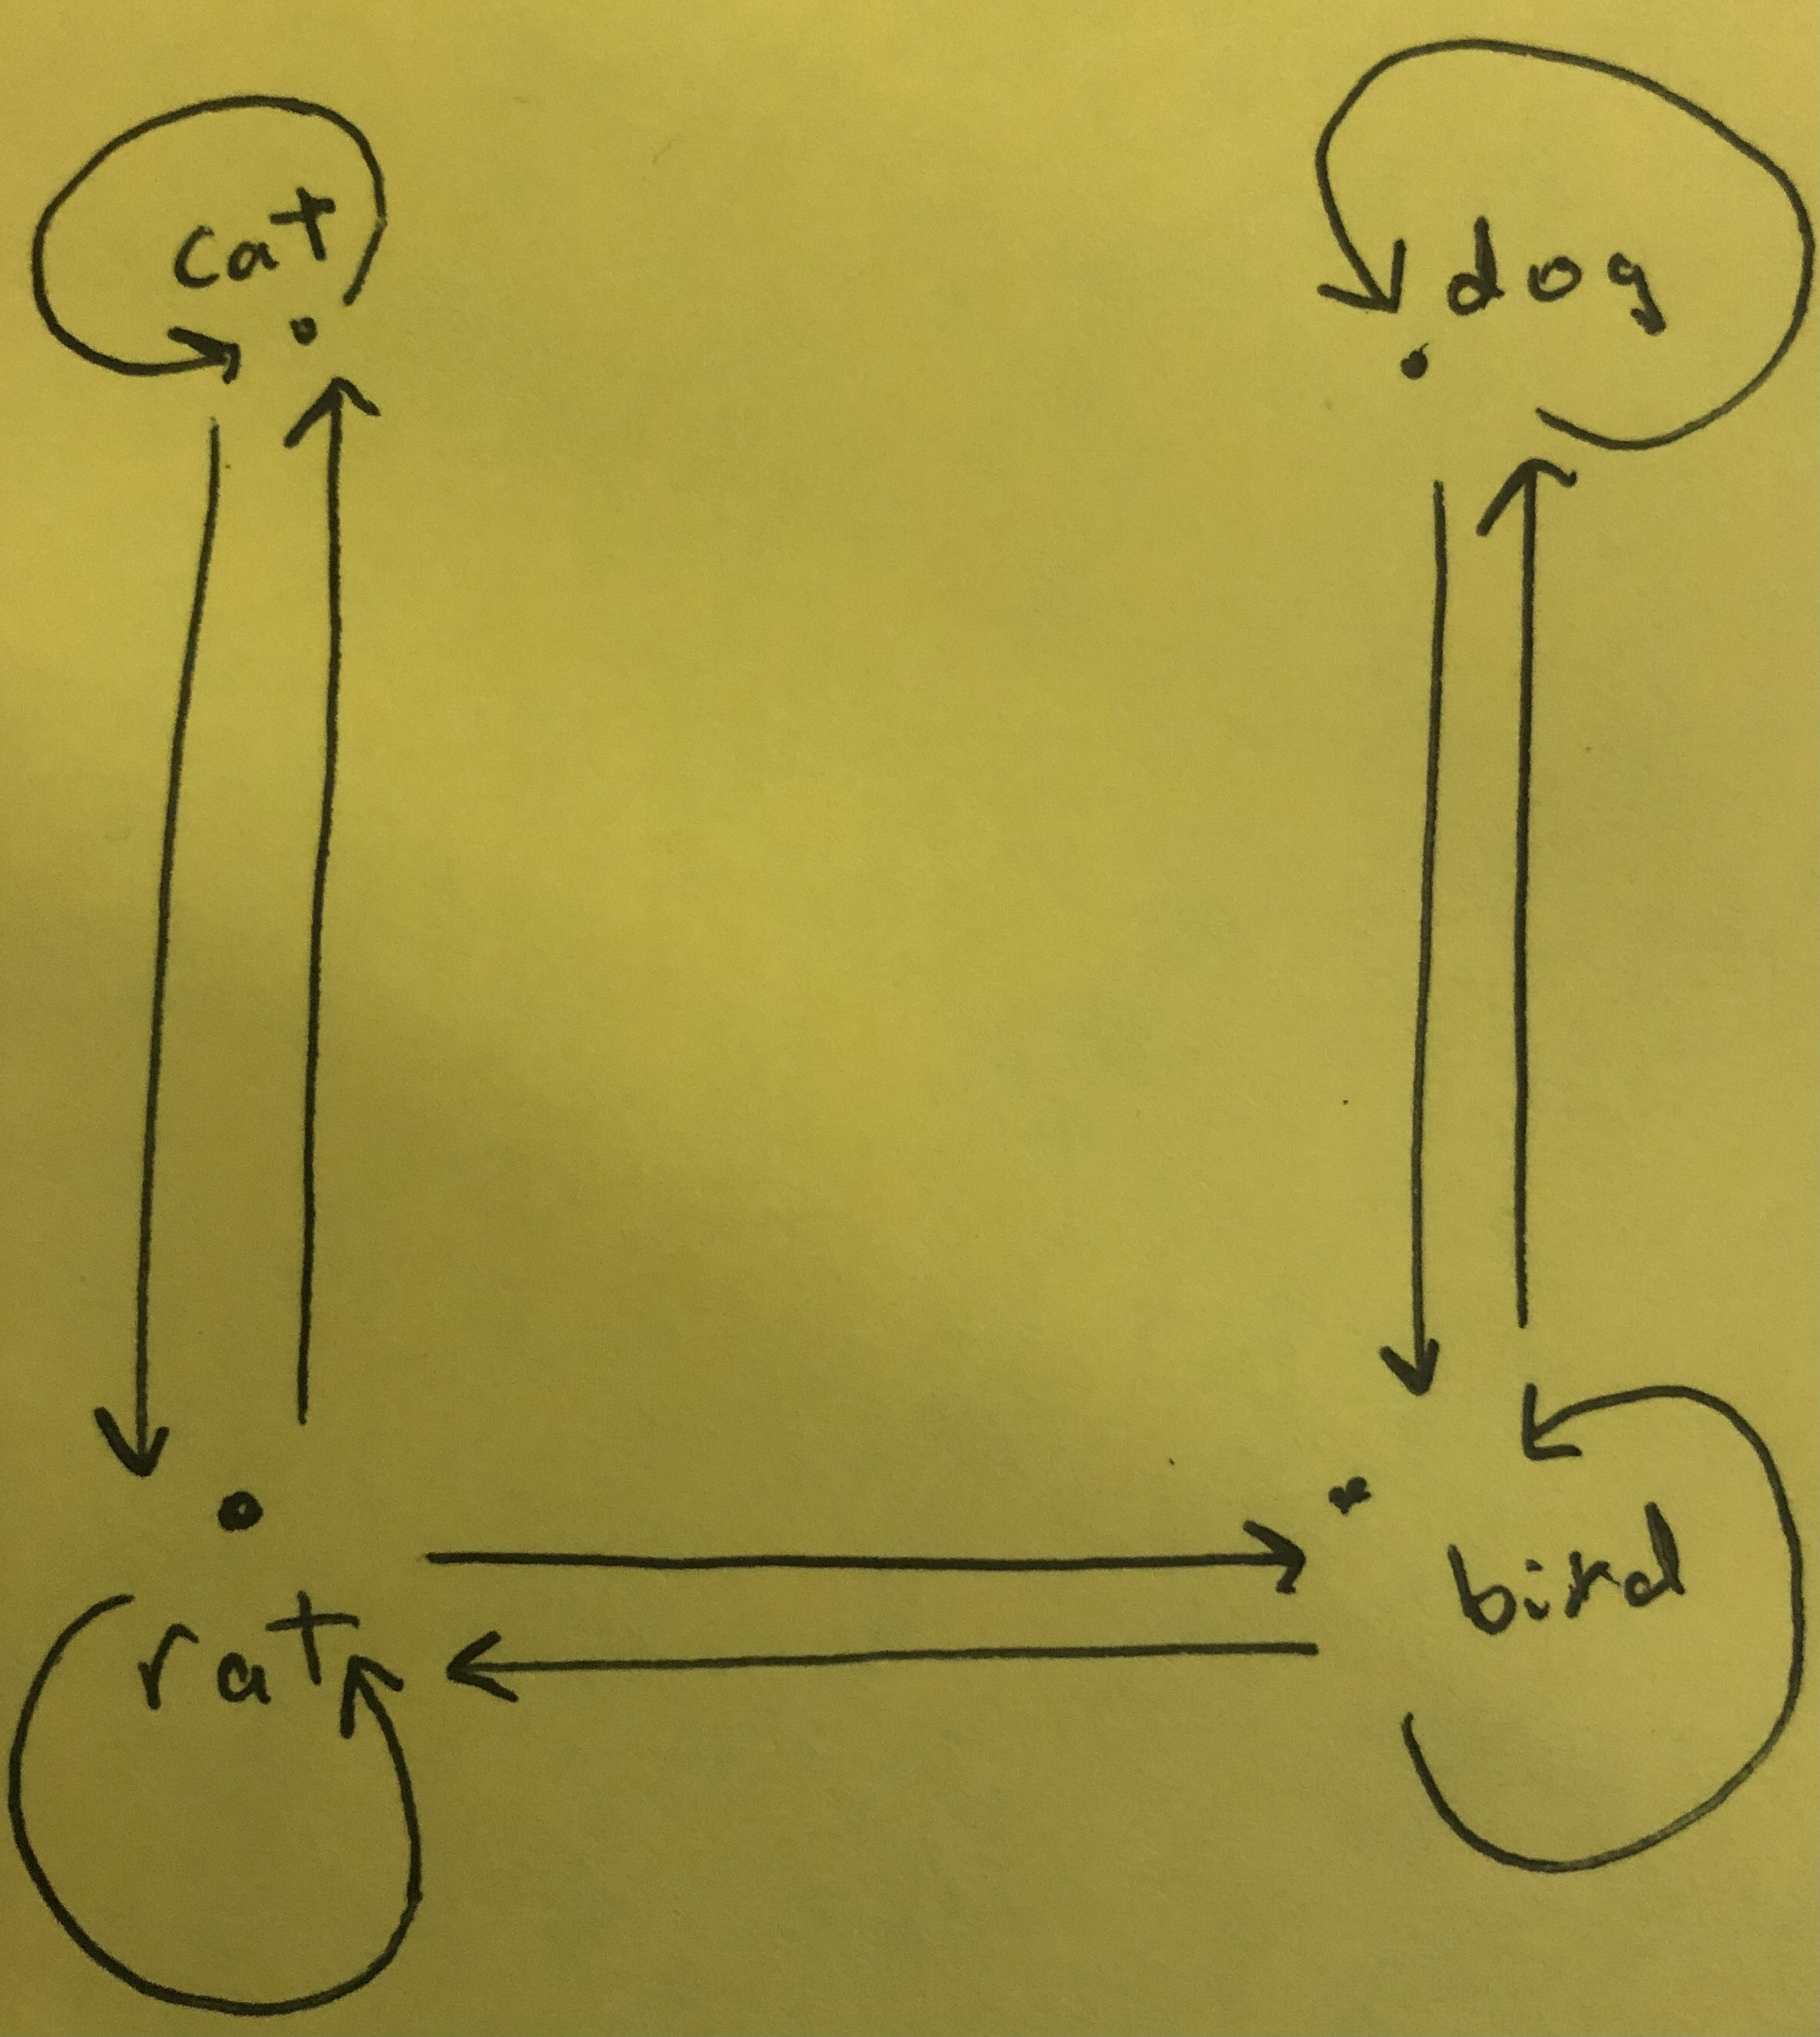
\includegraphics[scale=0.05]{image0.jpg}
\item  Is $R$ reflexive, symmetric, and/or transitive? \\
$R$ is reflexive as every element has every letter in common with itself. $R$ is also symmetric because if one element has a letter in common with another element, that other element also has that same letter in common with the first. $R$ is NOT transitive. While element 1 may have a letter in common with element 2 and element 2 might have a letter in common with element 3, these could be different letters meaning that element 1 may not be related to element 3, making it NOT transitive.
\end{enumerate}

\item Given a relation $R$ on a set $A$, prove that if $R$ is transitive, then so is $R^{-1}$. \\
For $R$ to be transitive on set $A$, substituting indexes for elements, $R$ must contain \{$(0,1),(1,2),(2,3)..(n,n+1),(0,n+1)$\}. Therefore, we know that $R^{-1}$ must contain \{$(n+1,n)..(3,2),(2,1),(1,0),(n+1,0)$\}. While in a different order, the first element is still related to the last, making the entire relation transitive. 

\item Suppose $R$ and $S$ are symmetric relations on a set $A$. Prove that $R \circ S $ is symmetric iff $R \circ S = S \circ R$. \\
Since both $R$ and $S$ are symmetric relations on a set $A$, if $R$ relates $p$ to $q$ and $S$ relates $q$ to $r$, then it is also true that $R$ relates $(q, p)$ and $S$ relates $(r,q)$. Assuming that $R \circ S = S \circ R$ is true, any value plugged into either $R \circ S$ or $S \circ R$ will result in the same value. From this, $R \circ S$ must be symmetric if the order can reversed and still lead to the same values. 

\item Prove or disprove: for any set $A$, there exists a relation $R$ on $A$ such that $R$ is both symmetric and antisymmetric. \\
Disproof. This relation would be true for any set with multiple elements as long as it is reflexive, meaning that each element is only related to itself. Sets with only one element cannot be antisymmetric as two elements not being related to one another unless they are equal is the definition of antisymmetricity and this is impossible with only one element.

\item Find all equivalence relations on \{1,2,3\}. \\
Reflexive: \{(1,1),(2,2),(3,3)\} \\
Transitive: \{(1,2),(2,3),(1,3)\} \\
Symmetric: \{(2,1),(3,2),(3,1)\} \\
All: \{(1,1),(2,2),(3,3),(1,2),(2,3),(1,3),(2,1),(3,2),(3,1)\}

\item Show that for $n$, $m \in Z+$, gcd($2^n -1, 2^m -1)= 2^{gcd(n,m)} - 1$. \\
The greatest common denominator of $2^n -1$  and $2^m -1$ must be a value that both $n$ and $m$ are divisible by. This same value would be what 2 is being raised to in the second part of the equation. By subtracing 1, the equation takes the same form as the first part.

\item Suppose $m,n, \in Z^+$ are relatively prime. Prove that for all $a,b \in Z$, $a \equiv b$ (mod $mn$) iff $a \equiv b$ (mod $m$) and $a \equiv b$ (mod $n$). \\
For the mod to result in a value that is not 0, the dividend and divisor must lack any common divisors. For $a \equiv b$ (mod $m$) to be true, there are two possible cases. $a$ and $b$ can share a common divisor with $m$ or both can not share a common divisor with $m$. The same is true for $a \equiv b$ (mod $n$) to be true. As long as these conditions both hold, $a \equiv b$ (mod $mn$) will be true for all $a$ and $b$ as long as $a$ and $b$ both do or both don't share a common divisor with $m$ and $n$.



\end{enumerate}
\end{document}
